\documentclass[12pt]{article}

\usepackage[utf8]{inputenc}
\usepackage{amsmath, amssymb, tikz, graphicx}

\title{Statistics 100A}
\author{Clayton Castro}
\date{March 31, 2025}

\begin{document}

\maketitle

\section*{Intro}

All physical laws are probabilistic.  
Einstein was against this interpretation; however, proponents such as Bohr, Heisenberg, and Schrödinger were ultimately proven correct by modern findings.

Artificial intelligence, natural language processing, robotics, etc., are all based on probabilistic frameworks.

Michael I. Jordan is a notable professor in this area.

Notable papers in the field:
\begin{itemize}
    \item AlexNet (Hinton's group)
    \item \textit{Attention Is All You Need}
\end{itemize}

Professor's comment from his time at Meta:
\begin{itemize}
    \item Did not prefer the probabilistic approach for scientific answers.
    \item Their models favored a deterministic approach.
\end{itemize}

Real-world applications:
\begin{itemize}
    \item ChatGPT
    \item Google PageRank
    \begin{itemize}
        \item Based on a Markov chain $\rightarrow$ stationary distribution.
        \item TikTok also applies this approach—very effective for increasing exposure to new content creators.
    \end{itemize}
    \item Monte Carlo algorithm
    \item Metropolis algorithm (considered the \#1 algorithm in scientific computing)
\end{itemize}

\section{Lecture 1}
\vspace{1em}
\noindent\textbf{\large April 2, 2025}

\paragraph{Monte Carlo Algorithm}
\begin{itemize}
    \item Used for high-dimensional integration and optimization.
    \item Very useful in AI.
\end{itemize}

\paragraph{AlphaGo}
\begin{itemize}
    \item Utilized a combination of "fast thinking" and "slow thinking".
    \item \textbf{Slow thinking}:
    \begin{itemize}
        \item Involves reasoning and planning.
        \item Uses Monte Carlo search and tree search.
    \end{itemize}
    \item \textbf{Fast thinking}:
    \begin{itemize}
        \item Involves intuition.
    \end{itemize}
\end{itemize}

\subsection{Sample Space}

\noindent
Experiment $\rightarrow$ Outcome $\rightarrow$ Number

\medskip

\noindent
Sample space $Q$: the set of all possible outcomes.

\medskip

\noindent
Event $A$:
\begin{itemize}
    \item A statement about the outcome (e.g., "greater than 4").
    \item A subset of the sample space (e.g., $\{5, 6\}$).
\end{itemize}

\noindent
Probability defined on an event:
\begin{equation}
    P(A) = \frac{|A|}{|Q|}
\end{equation}

% Lebegue measure \rightarrow probability equals counting

\section{Lecture 3}

A real population of people, under purely random sampling or imagined
population of equally likely possibilities.

\begin{center}
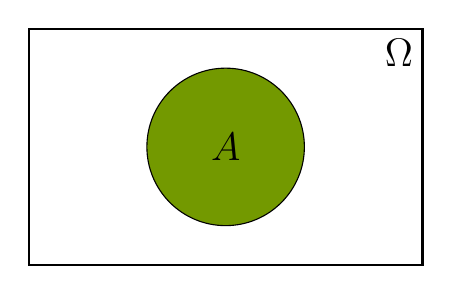
\begin{tikzpicture}
  \coordinate (center) at (2.5,1.5);
  \draw[thick] (0,0) rectangle (5,3);
  \filldraw[fill=lime!60!black, draw=black] (center) circle (1);
  \node at (center) {\Large $A$};
  \node at (4.7,2.7) {\Large $\Omega$};
\end{tikzpicture}
\[
    P(A) = \frac{|A|}{|\Omega|}
\]
\end{center}
Axiom 0.\\
Can always translate a problem into equally likely setting.

\begin{center}
\rule{4cm}{0.4pt}
\end{center}

\begin{center}
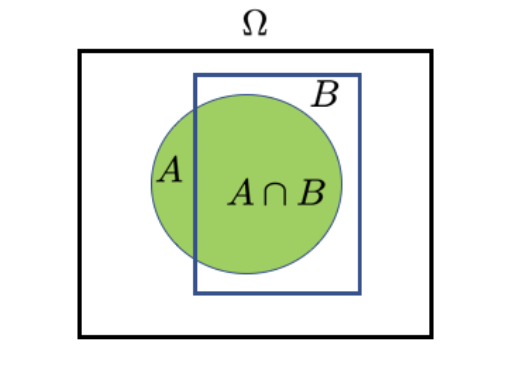
\includegraphics[width=0.4\textwidth]{conditional-probability.png}
\end{center}


\[
    P(A|B) = \frac{|A \cap B|}{|B|} = \frac{}{}
\]


\end{document}
